% CHKTEX-FILE 1
% \documentclass[letterpaper,10.5pt,twocolumn]{article}
\documentclass[letterpaper,10.5pt]{article}\usepackage[utf8]{inputenc}
\usepackage[T1]{fontenc}
\usepackage[english,spanish,mexico,es-lcroman]{babel}
% Standard packages
\usepackage{float}
\usepackage{ifthen}
\usepackage{xspace}
\usepackage{amsmath}
\usepackage{xstring}
\usepackage{wrapfig}
\usepackage{booktabs}
\usepackage{csquotes}
\usepackage{fancyhdr}
\usepackage{fancyvrb}
\usepackage{geometry}
\usepackage{graphicx}
\usepackage{lastpage}
\usepackage{listings}
\usepackage{multicol}
\usepackage{multirow}
\usepackage{tabularx}
\usepackage{algorithm}
\usepackage{textgreek}
\usepackage[justification=centering]{subcaption}
\usepackage{algpseudocode}
\usepackage[all]{nowidow}
\usepackage[inline]{enumitem}
\usepackage[usenames,dvipsnames]{xcolor}
% Packages to be loaded later
\usepackage{tikz}
\usepackage{cancel}
\usepackage{tcolorbox}
% Include fullpage images with \includepdf
% \usepackage{pdfpages}
% Referencing
\usepackage{varioref}
\usepackage{hyperref}
\usepackage[noabbrev,nameinlink,spanish]{cleveref}
\usepackage[square, comma, numbers, sort&compress]{natbib}


\newcommand{\lpar}{(}\newcommand{\rpar}{)} %CHKTEX 9
\newcommand{\IIC}{I\textsuperscript{2}C\xspace}
\newcommand{\GND}{\textsc{Gnd}\xspace}
\newcommand{\VCC}{\textsc{Vcc}\xspace}
\newcommand{\VDD}{\textsc{Vdd}\xspace}
\newcommand{\textbi}[1]{\textbf{\textit{#1}}}
\newcommand{\degreesC}[1]{%
	#1\textsuperscript{o}C\xspace{}%
}
\newcommand{\degreesF}[1]{%
	#1\textsuperscript{o}F\xspace{}%
}

% \newcommand{\VCC}{V\textsubscript{CC}\xspace{}}
% \newcommand{\GND}{\textsc{Gnd}\xspace{}}
% CHKTEX-FILE 26
% CHKTEX-FILE 36

\tcbuselibrary{most}
% \tcbuselibrary{listings,breakable}
% \usetikzlibrary{shadings,shadows}
% \usetikzlibrary{decorations.pathmorphing}
% \usetikzlibrary{patterns}
% \usetikzlibrary{spy}
% \usetikzlibrary{arrows.meta}

\newtcolorbox{importantbox}[1]{%
	enhanced,
	colback=red!5!white,%
	colframe=red!75!black,%
	fonttitle=\bfseries,%
	center title,
	title={#1},%
	drop fuzzy shadow
}

\newtcolorbox{marker}[1][]{%
	enhanced,
	before skip=2mm,after skip=3mm,
	boxrule=0.4pt,left=5mm,right=2mm,top=1mm,bottom=1mm,
	colback=yellow!50,
	colframe=yellow!20!black,
	sharp corners,rounded corners=southeast,arc is angular,arc=3mm,
%	underlay={%
%		\path[fill=tcbcolback!80!black] ([yshift=3mm]interior.south east)--++(-0.4,-0.1)--++(0.1,-0.2);
%		\path[draw=tcbcolframe,shorten <=-0.05mm,shorten >=-0.05mm] ([yshift=3mm]interior.south east)--++(-0.4,-0.1)--++(0.1,-0.2);
%		\path[fill=yellow!50!black,draw=none] (interior.south west) rectangle node[white]{\Huge\bfseries !} ([xshift=4mm]interior.north west);
%	},
	drop fuzzy shadow,#1
}

%CHKTEX-FILE 1
%CHKTEX-FILE 7
%CHKTEX-FILE 9
% Default fixed font does not support bold face
\DeclareFixedFont{\ttb}{T1}{txtt}{bx}{n}{8} % for bold
\DeclareFixedFont{\ttm}{T1}{txtt}{m}{n}{8}  % for normal

% Custom colors
\usepackage{color}
\definecolor{keywordsColor}{rgb}{0,0,0.5}
\definecolor{customColor}{rgb}{0.6,0,0}
\definecolor{stringColor}{rgb}{0,0.5,0}

% Code highlighting python
\renewcommand{\ttdefault}{pcr}
\lstset{
	language=Python,                              % the language of the code (can be overrided per snippet)
	backgroundcolor=\color{white},                % choose the background color
	basicstyle=\footnotesize\ttfamily,            % the size of the fonts that are used for the code
	breakatwhitespace=false,                      % sets if automatic breaks should only happen at whitespace
	breaklines=true,                              % sets automatic line breaking
	captionpos=t,                                 % sets the caption-position to bottom
	commentstyle=\color{gray},                    % comment style
	deletekeywords={},                            % if you want to delete keywords from the given language
%	escapeinside={\%*}{*)},                       % if you want to add LaTeX within your code
	extendedchars=true,                           % lets you use non-ASCII characters; for 8-bits encodings only, does not work with UTF-8
	frame=tb,                                     % adds a frame around the code
	keepspaces=true,                              % keeps spaces in text, useful for keeping indentation of code (possibly needs columns=flexible)
	keywordstyle=\color{keywordsColor}\bfseries,  % keyword style
	numbers=left,                                 % where to put the line-numbers; possible values are (none, left, right)
	numbersep=5pt,                                % how far the line-numbers are from the code
	numberstyle=\tiny\color{gray},                % the style that is used for the line-numbers
	rulecolor=\color{black},                      % if not set, the frame-color may be changed on line-breaks within not-black text (e.g. comments (green here))
	showspaces=false,                             % show spaces everywhere adding particular underscores; it overrides 'showstringspaces'
	showstringspaces=false,                       % underline spaces within strings only
	showtabs=false,                               % show tabs within strings adding particular underscores
	stepnumber=1,                                 % the step between two line-numbers. If it's 1, each line will be numbered
	stringstyle=\color{stringColor},              % string literal style
	tabsize=2,                                    % sets default tabsize to 2 spaces
	title=\lstname,                               % show the filename of files included with \lstinputlisting; also try caption instead of title
	columns=fixed,                                % Using fixed column width (for e.g. nice alignment)
	otherkeywords={self},                         % if you want to add more keywords to the set
	emphstyle=\color{customColor}\bfseries,       % Custom highlighting style
	emph={__init__,__main__,True,False,None},     % Custom highlighting keywords
	xleftmargin=1cm,                              % Left margin
	xrightmargin=1cm,                             % Right margin
	% Unicode compatibility
	inputencoding=utf8,
	literate={%
	            {Á}{{\'a}}1 {É}{{\'E}}1 {Í}{{\'I}}1 {Ó}{{\'O}}1 {Ú}{{\'U}}1%
	            {á}{{\'a}}1 {é}{{\'e}}1 {í}{{\'i}}1 {ó}{{\'o}}1 {ú}{{\'u}}1%
	            {À}{{\`A}}1 {È}{{\'E}}1 {Ì}{{\`I}}1 {Ò}{{\`O}}1 {Ù}{{\`U}}1%
	            {à}{{\`a}}1 {è}{{\`e}}1 {ì}{{\`i}}1 {ò}{{\`o}}1 {ù}{{\`u}}1%
	            {Ä}{{\"A}}1 {Ë}{{\"E}}1 {Ï}{{\"I}}1 {Ö}{{\"O}}1 {Ü}{{\"U}}1%
	            {ä}{{\"a}}1 {ë}{{\"e}}1 {ï}{{\"i}}1 {ö}{{\"o}}1 {ü}{{\"u}}1%
	            {Â}{{\^A}}1 {Ê}{{\^E}}1 {Î}{{\^I}}1 {Ô}{{\^O}}1 {Û}{{\^U}}1%
	            {â}{{\^a}}1 {ê}{{\^e}}1 {î}{{\^i}}1 {ô}{{\^o}}1 {û}{{\^u}}1% CHKTEX 19
	            {Ã}{{\~a}}1 {Ẽ}{{\~E}}1 {Ĩ}{{\~I}}1 {Õ}{{\~O}}1 {Ũ}{{\~U}}1 {Ñ}{{\~N}}1%
	            {ã}{{\~a}}1 {ẽ}{{\~e}}1 {ĩ}{{\~i}}1 {õ}{{\~o}}1 {ũ}{{\~u}}1 {ñ}{{\~n}}1%
	            {œ}{{\oe}}1 {Œ}{{\OE}}1 {æ}{{\ae}}1 {Æ}{{\AE}}1 {ß}{{\ss}}1%
	            {ç}{{\c c}}1 {Ç}{{\c C}}1 {ø}{{\o}}1 {å}{{\r a}}1 {Å}{{\r A}}1%
	            {€}{{\EUR}}1 {£}{{\pounds}}1 {×}{{\(\times\)}}1% CHKTEX 21
	            {°}{{\textsuperscript{o}}}1%
	            {¹}{{\textsuperscript{1}}}1%
	            {²}{{\textsuperscript{2}}}1%
	            {³}{{\textsuperscript{3}}}1%
	            {⁴}{{\textsuperscript{4}}}1% CHKTEX 19
	            {⁵}{{\textsuperscript{5}}}1% CHKTEX 19
	            {⁶}{{\textsuperscript{6}}}1% CHKTEX 19
	            {⁷}{{\textsuperscript{7}}}1% CHKTEX 19
	            {⁸}{{\textsuperscript{8}}}1% CHKTEX 19
	            {⁹}{{\textsuperscript{9}}}1% CHKTEX 19
	            {⁰}{{\textsuperscript{0}}}1% CHKTEX 19
%	            {A}{{\textAlpha}}1
	            {α}{{\textalpha}}1%
%	            {B}{{\textBeta}}1
	            {β}{{\textbeta}}1%
	            {Γ}{{\textGamma}}1
	            {γ}{{\textgamma}}1%
	            {Δ}{{\textDelta}}1
	            {δ}{{\textdelta}}1% CHKTEX 19
%	            {E}{{\textEpsilon}}1
	            {ϵ}{{\textepsilon}}1%
%	            {Z}{{\textZeta}}1
	            {ζ}{{\textzeta}}1%
%	            {H}{{\textEta}}1
	            {η}{{\texteta}}1%
	            {Θ}{{\textTheta}}1
	            {θ}{{\texttheta}}1%
%	            {I}{{\textIota}}1
	            {ι}{{\textiota}}1%
%	            {K}{{\textKappa}}1
	            {κ}{{\textkappa}}1%
	            {Λ}{{\textLambda}}1
	            {λ}{{\textlambda}}1%
%	            {M}{{\textMu}}1
	            {μ}{{\textmu}}1%
%	            {N}{{\textNu}}1
	            {ν}{{\textnu}}1%
	            {Ξ}{{\textXi}}1
	            {ξ}{{\textxi}}1%
%	            {O}{{\textOmikron}}1
%	            {o}{{\textomikron}}1%
	            {Π}{{\textPi}}1
	            {π}{{\textpi}}1%
%	            {P}{{\textRho}}1
	            {ρ}{{\textrho}}1%
	            {Σ}{{\textSigma}}1
	            {σ}{{\textsigma}}1%
%	            {T}{{\textTau}}1
	            {τ}{{\texttau}}1%
	            {ϒ}{{\textUpsilon}}1
	            {υ}{{\textupsilon}}1%
	            {Φ}{{\textPhi}}1
	            {ϕ}{{\textphi}}1%
%	            {X}{{\textChi}}1
	            {χ}{{\textchi}}1%
	            {Ψ}{{\textPsi}}1
	            {ψ}{{\textpsi}}1%
	            {Ω}{{\textOmega}}1
	            {ω}{{\textomega}}1%
	            {ζ}{{\varsigma}}1%
%	            {}{{\straightphi}}1%
%	            {}{{\scripttheta}}1%
%	            {}{{\straighttheta}}1%
%	            {}{{\straightepsilon}}1%
	         },
}

\lstdefinestyle{c_with_comments}%
{
	language     = c,
	morecomment  = [l]{//},
	morecomment  = [s]{/*}{*/},
	breaklines,
}

\lstdefinestyle{c_without_comments}%
{
	style        = c_with_comments,
	% numbers      = none,
	% keepspaces   = false,
	morecomment  = [l][\nullfont]{//},
	morecomment  = [is]{//}{\^^M},
	morecomment  = [is]{/*}{*/},
}

\lstdefinelanguage{conf}
{
	basicstyle=\ttfamily\small,
	columns=fullflexible,
	morecomment=[s][\color{Orchid}\bfseries]{[}{]},
	morecomment=[l]{\#},
	morecomment=[l]{;},
	commentstyle=\color{gray}\ttfamily,
	% morekeywords={},
	% otherkeywords={=,:},
	% keywordstyle={\color{Green}\bfseries}
}

% \captionsetup[lstlisting]{font={small,tt}}
\captionsetup[lstlisting]{%
	font={small},
}



\DefineVerbatimEnvironment{Verbatim}{Verbatim}{%
	fontsize=\footnotesize,%
	frame=leftline,%
	framesep=2em,    % separation between frame and text
}

\RecustomVerbatimCommand{\VerbatimInput}{VerbatimInput}{%
	fontsize=\footnotesize,
%	frame=lines,            % top and bottom rule only
	frame=leftline,         % left rule only
	numbers=left,           % Line numbers on the left
	numbersep=0.25em,       % Gap between numbers and verbatim lines
	xleftmargin=4em,        % Indentation to add at the start of each line
	xrightmargin=4em,       % Right margin to add after each line
	framesep=0.5em,         % separation between frame and text
	rulecolor=\color{Gray}, % Color of the lines
	labelposition=topline,  %
	samepage=false,         % When true, prevents verbatim environment from
	                        % being broken between pages
%	commandchars=\|\(\),    % escape character and argument delimiters for
	                        % commands within the verbatim
%	commentchar=*           % comment character
}


\hypersetup{
	hidelinks,
	colorlinks=true,
	linkcolor=Blue,
	filecolor=OliveGreen,
	urlcolor=RoyalPurple,
	pdfauthor={Mauricio Matamoros},
%	pdftitle={Práctica 0X – Fundamentos de Sistemas Embebidos},
% 	pdfsubject={The Subject},
% 	pdfkeywords={Some Keywords},
% 	pdfproducer={Latex with hyperref, or other system},
% 	pdfcreator={pdflatex, or other tool}
}

\captionsetup{%
	font=small
}

\geometry{%
	margin=2cm,
	% top=3cm,
	bottom=3cm,
	% left=2cm,
	% right=2cm,
	% inner=2cm,
	% outer=2cm,
	% headheight=,
	% footsep=,
	% footskip=,
}

\pagestyle{fancy}
\renewcommand{\headrulewidth}{0.0pt}
\lhead{}
\chead{}
\rhead{}
\lfoot{}
\cfoot{}
\rfoot{Página~\thepage~de~\pageref{LastPage}}

\crefname{table}{tabla}{tablas}
\Crefname{table}{Tabla}{Tablas}
\crefname{section}{sección}{secciones}
\Crefname{section}{Sección}{Secciones}
\crefname{subsection}{subsección}{subsecciones}
\Crefname{subsection}{Subsección}{Subsecciones}
\crefname{listing}{código de ejemplo}{códigos de ejemplo}
\Crefname{listing}{Código de Ejemplo}{Códigos de Ejemplo}
\renewcommand*{\lstlistingname}{Código ejemplo}


\hypersetup{
	hidelinks,
	pdfauthor={Mauricio Matamoros},
	pdftitle={Programa 02 – Fundamentos de Sistemas Embebidos},
% 	pdfsubject={The Subject},
% 	pdfkeywords={Some Keywords},
% 	pdfproducer={Latex with hyperref, or other system},
% 	pdfcreator={pdflatex, or other tool}
}


\author{\footnotesize Autor: José Mauricio Matamoros de Maria y Campos}
\title{Programa 2:\\Control remoto de una simulación de puerto GPIO de la Raspberry Pi via WiFi y servidor web\\
{\large Fundamentos de Sistemas Embebidos}}
\date{}


% Document body
\begin{document}
\maketitle

% %% %%%%%%%%%%%%%%%%%%%%%%%%%%%%%%%%%%%%%%%%%%%%%%%%%%%%%%%%%%
% objective.tex
%
% Author:  Mauricio Matamoros
% License: MIT
%
% %% %%%%%%%%%%%%%%%%%%%%%%%%%%%%%%%%%%%%%%%%%%%%%%%%%%%%%%%%%%

\section{Objetivo}%
\label{sec:objective}
El alumno aprenderá a leer e interpretar señales analógicas discretizadas con un microcontrolador.

% %% %%%%%%%%%%%%%%%%%%%%%%%%%%%%%%%%%%%%%%%%%%%%%%%%%%%%%%%%%%
% materials.tex
%
% Author:  Mauricio Matamoros
% License: MIT
%
% %% %%%%%%%%%%%%%%%%%%%%%%%%%%%%%%%%%%%%%%%%%%%%%%%%%%%%%%%%%%

%!TEX root = ../main.tex
%!TEX root = ../references.bib

\section{Material}%
\label{sec:material}
\begin{enumerate}[noitemsep]
	\item Plataforma:
	\begin{itemize}[nosep]
		\item Computadora con sistema operativo Linux, o
		\item Máquina virtual con sistema operativo Raspbian, o
		\item Raspberry Pi con sistema operativo Raspbian
	\end{itemize}
	\item Interprete de Python 3.5 instalado.
	\item Código del programa anterior.
\end{enumerate}

\begin{importantbox}{\bfseries ADVERTENCIA}
Cuando se configura un sistema Linux como punto de acceso inalámbrico con DHCP, éste pierde la capacidad de utilizar la tarjeta inalámbrica para conectarse a internet via inalámbrica.

Por este motivo se recomienda que los programas se prueben en una máquina virtual o en una Raspberry Pi si no se sabe cómo revertir este proceso.
\end{importantbox}

\textbf{Nota:} Si se cuenta con una Raspberry Pi sin WiFi integrado (e.j~Raspberry Pi2), se precisará de un adaptador WiFi USB compatible para la misma.

% %% %%%%%%%%%%%%%%%%%%%%%%%%%%%%%%%%%%%%%%%%%%%%%%%%%%%%%%%%%%
% steps.tex
%
% Author:  Mauricio Matamoros
% License: MIT
%
% %% %%%%%%%%%%%%%%%%%%%%%%%%%%%%%%%%%%%%%%%%%%%%%%%%%%%%%%%%%%
%!TEX root = ../practica.tex
%!TEX root = ../references.bib

% CHKTEX-FILE 1
% CHKTEX-FILE 13
% CHKTEX-FILE 46

\section{Instrucciones}%
\label{sec:instructions}
\begin{enumerate}[noitemsep]
	\item Alambre el circuito mostrado en las \Cref{fig:circuit-dc,fig:circuit-ac}.
	\item Realice los programas de la \Cref{sec:step3}
 	\item Analice los programas de la \cref{sec:step3} y realice los experimentos propuestos en la \cref{sec:experiments}.
 	% y con los resultados obtenidos responda el cuestionario de la \cref{sec:questionnaire}.
\end{enumerate}

% %% %%%%%%%%%%%%%%%%%%%%%%%%%%%%%%%%%%%%%%%%%%%%%%%%%%%%%%%%%%
% step-1.tex
%
% Author:  Mauricio Matamoros
% License: MIT
%
% %% %%%%%%%%%%%%%%%%%%%%%%%%%%%%%%%%%%%%%%%%%%%%%%%%%%%%%%%%%%
%!TEX root = ../practica.tex
%!TEX root = ../references.bib

% CHKTEX-FILE 1
% CHKTEX-FILE 13
% CHKTEX-FILE 46

\subsection{Implementación un controlador On/Off}%
\label{sec:step-1}

Alambre cuidadosamente los circuitos de las prácticas \href{https://github.com/kyordhel/FSEm/tree/master/practica06}{6} y \href{https://github.com/kyordhel/FSEm/tree/master/practica07}{7} para crear un circuito AC-DC optoacoplado completo para control cerrado de temperatura usando un foco incandescente operado con un LM35 y un circuito de variación de fase mediante detección de cruce por cero.
El circuito completo alambrado debe verse como el de la \Cref{fig:circuit-full}.

\medskip

\begin{importantbox}{\large Importante}
	\begin{center}
		Asegúrese de verificar con un multímetro que el circuito de AC está debidamente aislado y que no se tienen valores mayores a 5V en el segmento de DC.
		De otro modo podría quemar su Arduino y su Raspberry Pi.
	\end{center}
\end{importantbox}

\medskip

\begin{figure}
	\centering
	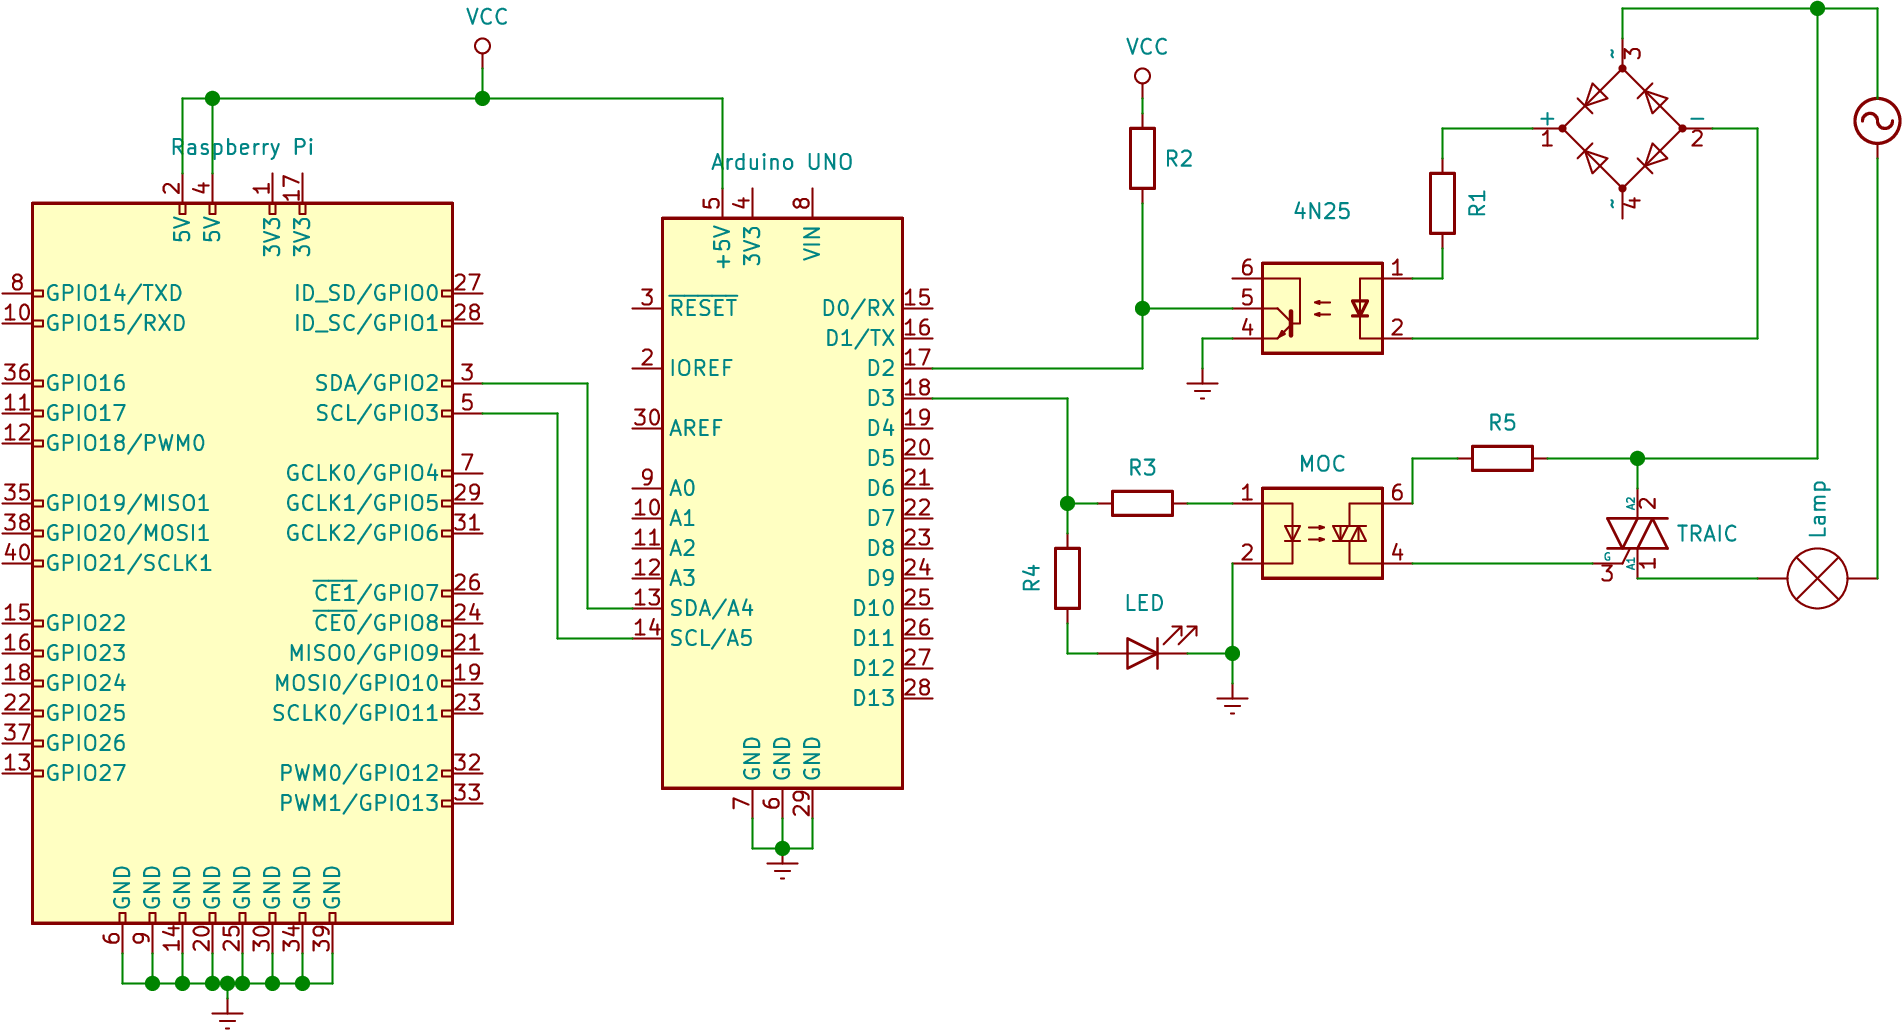
\includegraphics[width=0.85\linewidth,height=6cm,keepaspectratio]{img/circuit-full.png}
	\caption{Circuito AC-DC optoacoplado completo para control cerrado de temperatura.}%
	\label{fig:circuit-full}
\end{figure}

De acuerdo con el alambrado de la \Cref{fig:circuit-full}, el Arduino ha de realizar tres funciones:
\begin{enumerate*}[label=\roman*\rpar]
	\item digitalización del valor de temperatura analógico sensado por el LM35,
	\item la detección del cruce por cero de la onda sinusoidal de la línea eléctrica,
	y
	\item la modulación de potencia del foco incandescente mediante variación de fase ajustada por el retardo en el disparo del TRIAC.
\end{enumerate*}
Al igual que en las prácticas anteriores, el Arduino estará configurado como dispositivo esclavo y estas operaciones estarán al servicio del dispositivo maestro: la Raspberry Pi.
Así, una operación de lectura proporcionará al dispositivo maestro la temperatura sensada, mientras que una operación de escritura enviará la potencia con la que encenderá el foco como un valor flotante entre 0 y 100, quedando a cargo del Arduino el cálculo de la variación de fase y la sincronización de las operaciones de hardware.

\paragraph{Nota:} La implementación del código del Arduino se deja a cargo del estudiante.

\medskip

Se puede proceder entonces a revisar el código de control que se ejecutará en la Raspberry Pi.
En este caso se implementará un controlador On/Off tal como se describe en la \Cref{sec:control-onoff}.

Lo primero es incluir los paquetes necesarios y proveer cuatro parámetros importantes:
\begin{enumerate*}[label=\arabic*\rpar]
	\item la dirección del dispositivo esclavo,
	\item la temperatura deseada,
	\item el umbral o valor de encendido,
	y
	\item el umbral o valor de apagado
\end{enumerate*}
tal como se muestra en el \Cref{lst:controller-code-params}.

\begin{minipage}{\linewidth}%
\lstinputlisting[%
	language=python,
	caption={\texttt{controller-on-off.py:9--20} --- Parámetros},
	label={lst:controller-code-params},
	firstline=9,
	lastline=20]{src/controller-on-off.py}
\end{minipage}

El controlador con los parámetros descritos anteriormente requerirá de dos funciones auxiliares: \emph{readTemperature} (véase \Cref{lst:controller-code-read}) y \emph{writePower} (véase \Cref{lst:controller-code-write}).
La primer función corresponde a una operación de lectura en la cual el Arduino proporcionará la temperatura registrada por el sensor en grados centígrados codificado como un valor flotante (4 bytes en little endian).
La segunda función es una operación de escritura en la cual la Raspberry Pi proporcionará al arduino el factor de potencia de 0 a 100 codificada como un valor flotante (4 bytes en little endian).

\begin{minipage}{\linewidth}%
\lstinputlisting[%
	language=python,
	caption={\texttt{controller-on-off.py:26--36} --- Función \emph{readTemperature}},
	label={lst:controller-code-read},
	firstline=26,
	lastline=36]{src/controller-on-off.py}
\end{minipage}

\begin{minipage}{\linewidth}%
\lstinputlisting[%
	language=python,
	caption={\texttt{controller-on-off.py:38--45} --- Función \emph{writePower}},
	label={lst:controller-code-write},
	firstline=38,
	lastline=45]{src/controller-on-off.py}
\end{minipage}

Por último queda revisar la implementación del controlador mostrada en el \Cref{lst:controller-onoff-code}.
El control de temperatura se ejecuta en un bucle infinito de tres partes dentro de la función principal \emph{main}.
\begin{enumerate*}[label=\arabic*\rpar]
	\item Primero se lee la temperatura en °C del arduino,
	\item después esta se compara con los umbrales.
	Si la temperatura es menor al valor de encendido la lámpara se enciende a máxima potencia y permanecerá encendida hasta que se supera el valor de apagado.
	Por último,
	\item el controlador entra en un estado de espera (1 segundo) donde no se realiza ninguna acción.
\end{enumerate*}
En cualquier otro caso no se hace nada.

\begin{minipage}{\linewidth}%
\lstinputlisting[%
	language=python,
	caption={\texttt{controller-on-off.py:47--67} --- Función \emph{main}},
	label={lst:controller-onoff-code},
	linerange={47-47,51-52,54-55,57-67} %CHKTEX 8
	]{src/controller-on-off.py}
\end{minipage}
% %% %%%%%%%%%%%%%%%%%%%%%%%%%%%%%%%%%%%%%%%%%%%%%%%%%%%%%%%%%%
% step-2.tex
%
% Author:  Mauricio Matamoros
% License: MIT
%
% %% %%%%%%%%%%%%%%%%%%%%%%%%%%%%%%%%%%%%%%%%%%%%%%%%%%%%%%%%%%
%!TEX root = ../practica.tex
%!TEX root = ../references.bib

% CHKTEX-FILE 1
% CHKTEX-FILE 13
% CHKTEX-FILE 46
\subsection{Paso 2: Configuración de comunicaciones \IIC}%
\label{sec:step3}
Primero ha de configurarse la Raspberry Pi para funcionar como dispositivo maestro o \emph{master} en el bus \IIC.
Para esto, inicie la utilidad de configuración de la Raspberry Pi con el comando

\begin{Verbatim}
# raspi-config
\end{Verbatim}

\noindent y seleccione la opción 5: Opciones de Interfaz (\emph{Interfacing Options}) y active la opción \texttt{P5} para habilitar el \IIC.

A continuación, verifique que el puerto \IIC no se encuentre en la lista negra.
Edite el archivo \\\texttt{/etc/modprobe.d/raspi-blacklist.conf} y revise que la línea \texttt{blacklist spi-bcm2708} esté comentada con \#.

% $ cat /etc/modprobe.d/raspi-blacklist.conf
\begin{lstlisting}[
	language=conf,
	caption={/etc/modprobe.d/raspi-blacklist.conf},
	label={lst:raspi-blacklist.conf},
	numbers=none
]
# blacklist spi and i2c by default (many users don't need them)
# blacklist i2c-bcm2708
\end{lstlisting}

Como paso siguiente, se habilita la carga del driver \IIC.
Esto se logra agregando la línea \texttt{i2c-dev} al final del archivo \texttt{/etc/modules} si esta no se encuentra ya allí.

Por último, se instalan los paquetes que permiten la comunicación mediante el bus \IIC y se habilita al usuario predeterminado \emph{pi} (o cualquier otro que se esté usando) para acceder al recurso.

\begin{Verbatim}
# apt-get install i2c-tools python-smbus
# adduser pi i2c
\end{Verbatim}

Reinicie la Raspberry Pi y pruebe la configuración ejecutando \texttt{i2cdetect -y 1} para buscar dispositivos conectados al bus \IIC.
Debería ver una salida como la siguiente:

\begin{Verbatim}
\$ i2cdetect -y 1
     0  1  2  3  4  5  6  7  8  9  a  b  c  d  e  f
00:          -- -- -- -- -- -- -- -- -- -- -- --
10: -- -- -- -- -- -- -- -- -- -- -- -- -- -- --
20: -- -- -- -- -- -- -- -- -- -- -- -- -- -- --
30: -- -- -- -- -- -- -- -- -- -- -- -- -- -- --
40: -- -- -- -- -- -- -- -- -- -- -- -- -- -- --
50: -- -- -- -- -- -- -- -- -- -- -- -- -- -- --
60: -- -- -- -- -- -- -- -- -- -- -- -- -- -- --
70: -- -- -- -- -- -- -- --
\end{Verbatim}

% %% %%%%%%%%%%%%%%%%%%%%%%%%%%%%%%%%%%%%%%%%%%%%%%%%%%%%%%%%%%
% step-3.tex
%
% Author:  Mauricio Matamoros
% License: MIT
%
% %% %%%%%%%%%%%%%%%%%%%%%%%%%%%%%%%%%%%%%%%%%%%%%%%%%%%%%%%%%%

%!TEX root = ../main.tex
%!TEX root = ../references.bib

\subsection{Paso 3: Display de siete segmentos}%
\label{sec:step4}
El código mostrado en \Cref{src:bcd} muestra cómo se operaría un display de siete segmentos mediante una controladora TTL 74LS47 utilizando la Raspberry Pi.

\smallskip
\lstinputlisting[%
	language=Python,
	linerange={19-51}, % chktex 8
	caption={\texttt{bcd.py}},
	label={src:bcd}
]{src/bcd.py}
\smallskip

Estudie el código y véalo en funcionamiento, ejecutándolo de la siguiente manera:
\begin{Verbatim}[fontsize=\footnotesize]
./bcd.py
\end{Verbatim}



% %% %%%%%%%%%%%%%%%%%%%%%%%%%%%%%%%%%%%%%%%%%%%%%%%%%%%%%%%%%%
% appspecs.tex
%
% Author:  Mauricio Matamoros
% License: MIT
%
% %% %%%%%%%%%%%%%%%%%%%%%%%%%%%%%%%%%%%%%%%%%%%%%%%%%%%%%%%%%%

%!TEX root = ../main.tex
%!TEX root = ../references.bib

\section{Programas}%
\label{sec:programs}

Integre el código del Programa 1 en un archivo python llamado \texttt{led\_manager.py} y que ofrezca las siguientes funciones:
\begin{enumerate}
	\item{} [2 pts] Encendido del del 1--7 al presionar el boton adecuado.

	\item{} [2 pts] Desplegado de la marquesina izquierda al presionar el boton adecuado.\footnote{Una marquesina izquiera muestra el corrimiento circular hacia la izquierda del led menos significativo (i.e.~de derecha o menos significativo a izquierda o más significativo), manteniendo únicamente un led encendido en todo momento.}

	\item{} [2 pts] Desplegado de la marquesina derecha al presionar el boton adecuado.\footnote{Una marquesina derecha muestra el corrimiento circular hacia la derecha del led más significativo (i.e.~izquierda o más significativo a de derecha o menos significativo), manteniendo únicamente un led encendido en todo momento.}

	\item{} [2 pts] Desplegado de la marquesina tipo ping-pong al presionar el boton adecuado.\footnote{Una marquesina tipo ping-pong o de rebote muestra el corrimiento hacia la derecha del led más significativo hasta alcanzar el led menos significativo, momento en el que se invierte la dirección del corrimiento y así sucesivamente, dando la impresión de que el led \enquote{rebota} en los extremos.}

	\item{} [2 pts] Desplegado del dígito correcto en el display de 7 segmentos al presionar el boton correspondiente
\end{enumerate}
\section{Especificaciones técnicas de los programas}%
\label{sec:programs-specs}
\begin{itemize}[noitemsep]
	\item No utilice paquetes adicionales.
	\item El código deberá ser ejecutable con Python versión 3.5 o posterior.
	\item Todos los programas deberán comenzar con la línea de intérprete o \emph{she-bang} correspondiente
	\item Todos los programas deberán tener el nombre del autor de la forma:

\begin{lstlisting}[language=python]
# Author: Nombre del Alumno
\end{lstlisting}
	\item En los videos-evidencia deberá observarse claramente cómo el alumno controla remotamente desde la interfaz de usuario al simulador de la RaspBerry Pi (ej.~desde su celular o desde otra máquina virtual).

	\item Incluya sólo los videos y el código fuente de los programas \textbi{sin librerías ni paquetes}.
	\item Los archivos de código python deberán estar en raíz \texttt{./}.
	\item Los videos-evidencia deberán estar en el subdirectorio \texttt{./vid/}.
	\item Los videos-evidencia deberán durar no más de 60 segundos, incluir sólo la ventana del simulador y contar únicamente con \emph{stream} de video comprimido con \emph{codec} h.264 a \(15fps\) con una resolución máxima de \(1280 \times 720\) y con un tamaño máximo de 3MB por archivo (velocidad de datos aproximada de \(1500kbps\))\footnote{\texttt{ffmpeg -i input -an -vf scale=-1:720 -c:v libx264 -crf 28 -r 15 -preset veryslow hicm\_osblink8.mp4}}.
	\item Los entregables deberán estar empaquetados en un archivo comprimido de nombre \texttt{[prefijo]\_p02} donde \texttt{[prefijo]\_p02} corresponde a los primeros 4 caracteres de la CURP del alumno, por ejemplo \texttt{hicm\_p01.zip}.
	Los formatos aceptables son \emph{7z}, \emph{rar}, \emph{tar.bz2}, \emph{tar.gz} y \emph{zip}.
\end{itemize}


\cleardoublepage%
\appendix

% %% %%%%%%%%%%%%%%%%%%%%%%%%%%%%%%%%%%%%%%%%%%%%%%%%%%%%%%%%%%
% appendices.tex
%
% Author:  Mauricio Matamoros
% License: MIT
%
% %% %%%%%%%%%%%%%%%%%%%%%%%%%%%%%%%%%%%%%%%%%%%%%%%%%%%%%%%%%%

% CHKTEX-FILE 1
% CHKTEX-FILE 46

\section{El archivo \texttt{temperature.py}}%
\label{sec:temperature-py}
% \setlength{\columnsep}{1cm}
% \begin{multicols}{2}
\lstinputlisting[%
	firstline=17,
	basicstyle=\scriptsize\ttfamily,
	xleftmargin=0cm,
	xrightmargin=0cm,
	frame=none,
	label=lst:temperature-py,
	caption=Archivo temperature.py
]{src/temperature.py}
% \end{multicols}


\end{document}
